\documentclass[titlepage,12 pt]{article} 

\usepackage{amsmath} 
\usepackage{amssymb} 
\usepackage{amsfonts} 
\usepackage{cancel}
\usepackage{graphics,graphicx}
\usepackage[font=small,labelfont=bf]{caption}


\newcommand{\N}{{\mathbb N}}
\newcommand{\Z}{{\mathbb Z}}
\newcommand{\Q}{{\mathbb Q}}
\newcommand{\R}{{\mathbb R}}
\newcommand{\C}{{\mathbb C}}
\newcommand{\ds}{\displaystyle} 
\newcommand{\E}{\mathbb{E}}
\DeclareMathOperator*{\argmax}{arg\,max}
\DeclareMathOperator*{\mode}{mode}

\parindent 0 cm 
\parskip 0.6 cm 
\oddsidemargin 0.15 cm 
\textwidth 16 cm 
\topmargin -2 cm
\textheight 23 cm 

\renewcommand{\baselinestretch}{1.2}


\begin{document} 

\begin{titlepage}

\begin{center}

\includegraphics[height=2 cm]{St-Lawrence_Logo.png}
\vspace{1 cm}

\Large{
{\bf The Gumbel and Logistic Distributions}
}
\vspace{1 cm}

\begin{center}
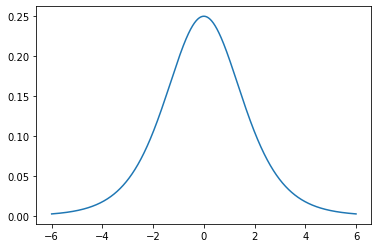
\includegraphics[height=6 cm]{Logistic-f.png}
\end{center}
\vspace{1 cm}

{\bf Probability and Statistics 201-BNM-LW}
\vspace{5 mm}

\large{

{\bf IA Project $-$ Winter Semester 2024}

{\bf presented to}

\textbf{Vincent Carrier}

\textbf{by Charles-Edward Gagnon, Raphaël Parenteau and Noah Vaillancourt}

}

\end{center}

\end{titlepage}

\tableofcontents

\pagebreak

\section{Introduction}

\subsection{Context of Gumbel Distribution}

Let $X_1, X_2,..., X_n$ be i.i.d. and $X_i\sim \mathcal{E}\text{xp}(\lambda)$. If $Y_n=X_{(n)}-\ln{n}$, then
\begin{align*}
G_{n}(y)&=P(Y_n\le y) \\[2mm]
&=P(X_{(n)}-\ln{n}\le y)\\[2mm]
&=P(X_1-\ln{1}\le y)\;P(X_2-\ln{2}\le y)\;...\;P(X_n-\ln{n}\le y) \\[2mm]
&=P(X_1\le y+\ln{1})\;P(X_2\le y+\ln{2})\;...\;P(X_n\le y+\ln{n}) \\[2mm]
&=\left[ F(y+\ln{n}) \right]^{n} \\[2mm]
&=\left( 1-e^{-\lambda(y+\ln{n})} \right)^{n} \\[2mm]
&=\left( 1-e^{-\lambda y}e^{-\lambda\ln{n}} \right)^{n} \\[2mm]
&=\left( 1-e^{-\lambda y}e^{\ln{(1/n^{\lambda})}} \right)^{n} \\[2mm]
&=\left( 1-\frac{e^{-\lambda y}}{n^{\lambda}} \right)^{n} \\[2mm]
\end{align*}
Set $\lambda=1$ \\
(See Appendix for proof of the limit of $(1+t/n)^n=e^t \quad n\to\infty$)
\begin{align*}
\lim_{n\to\infty} G_{n}(y) &=\lim_{n\to\infty} \left( 1-\frac{e^{-y}}{n} \right)^{n} \\[2mm]
&= \lim_{n\to\infty} \left( 1+ \frac{-e^{-y}}{n} \right)^{n} \\[2mm]
&= e^{-e^{-y}}
\end{align*}

This is the distribution function $F(x)$ of the standard Gumbel distribution. It gives the probability that the maximum value of i.i.d exponentially distributed random variables minus a correction factor is smaller or equal to a given value. As such, the Gumbel Distribution is used to model the distribution of the maximum value of a random variable.

\section{Density and Distribution Functions}

When $X\sim \mathcal{G}\text{umbel}(\mu,\beta)$, the density function is given by 

\[\ds f(x)=\frac{1}{\beta}e^{-(z+e^{-z})} \quad \text{ where } z=\frac{x-\mu}{\beta}.
\]

The standard Gumbel distribution is given by
$$ X \sim \mathcal{G}\text{umbel}(0,1) \quad f(x) = e^{-(x + e^{-x})} \quad \text{ for } x \in \R $$

The function $f(x)$ given above is indeed a density function since
\begin{align*}
\int_{D_x} f(x) \, dx & = \lim_{(s,t)\to(-\infty,\infty)} \int_{s}^{t} e^{-(x+e^{-x})} \, dx \\[3 mm]
&= \lim_{s\to-\infty} \int_{s}^{0} e^{-x}e^{-e^{-x}} \, dx + \lim_{t\to\infty} \int_{0}^{t} e^{-x}e^{-e^{-x}} \, dx
& \boxed{\begin{aligned}u &= -e^{-x} \\
             du &= e^{-x} \, dx \end{aligned}} \\[3 mm]
&= \lim_{s\to-\infty} \int_{-e^{-s}}^{0} e^{u} \, du + \lim_{t\to\infty} \int_{0}^{-e^{-t}} e^{u} \, du \\[3 mm]
&= \lim_{s\to-\infty}  e^{u} \mid|_{-e^{-s}}^{0} + \lim_{t\to\infty} e^{u} \mid|_{0}^{-e^{-t}} \\[3 mm]
&= \lim_{s\to-\infty} (e^0-e^{-e^{-s}}) + \lim_{t\to\infty} (e^{-e^{-t}}-e^0) \\[3 mm]
&=1 \\
\end{align*}

The distribution function of the standard Gumbel distribution is given by
\begin{align*}
    F(x)& =P(X\leq x) \\[3mm]
    &=\lim_{t\to-\infty} \int_{t}^{x} e^{-(u + e^{-u})} \, du \\[3mm]
    &= \lim_{t\to-\infty} \int_{t}^{x} e^{-u}e^{-e^{-u}} \, du
& \boxed{\begin{aligned}v &= -e^{-u} \\
             dv &= e^{-u} \, du \end{aligned}} \\[3 mm]
    &= \lim_{t\to-\infty} \int_{-e^{-t}}^{-e^{-x}} e^{v} \, dv \\[3mm]
    &= \lim_{t\to-\infty} e^v \mid|_{-e^{-t}}^{-e^{-x}} \\[3mm]
    &= \lim_{t\to-\infty} (e^{-e^{-x}}-e^{-e^{-t}}) \\[3mm]
    &= e^{-e^{-x}} \\
\end{align*}
When $ X \sim \mathcal{G}\text{umbel}(\mu,\beta) $, the distribution function is given by
$$ f(x)=e^{-e^{-(x-\mu})/\beta} $$

\section{Expected Value and Variance}

The expected value of the standard Gumbel distribution is given by
\begin{align*}
E(X)&= \int_{-\infty}^{\infty} xe^{-(x + e^{-x})} \, dx \\[3mm]
    &= \int_{-\infty}^{\infty} xe^{-x}e^{-e^{-x}} \, dx
    & \boxed{\begin{aligned}y &= e^{-x} \\
             dy &= -e^{-x} \, dx \\
             lny &= -x \end{aligned}} \\[3 mm]
    &= \int_{0}^{\infty} e^{-y} \ln{y} \, dy \\[3mm]
\end{align*}

This integral converges to the Euler-Mascheroni constant, $\gamma$ . This constant, often referred to as Euler's constant, for Leonhard Euler was the first to describe it in 1734, is defined as the limiting difference between the harmonic series and the natural logarithm.
\\ 
To support this definition of $\gamma$, let $S_{n_1}$ be the harmonic series:
\begin{equation*}
 S_{n_1} = \sum_{k=1}^{n} \frac{1}{k} = \frac{1}{1} + \frac{1}{2} + \dots + \frac{1}{n}   
\end{equation*}



And let $S_{n_2}$ be the natural logarithm expressed as an integral bounded by 1 and n:
\begin{align*}
S_{n_2} & = \ln{n} \\[3 mm]
              &= \int_{1}^{n} \frac{1}{x} \,dx
\end{align*}
              
Consider $S_N$, the difference between $S_{n_1}$ and $S_{n_2}$ :
\begin{align*}
    S_{N}& = S_{n_1} - S_{n_2}
    \\[2 mm] 
    &= \sum_{k=1}^{n} \frac{1}{k} -\int_{1}^{n} \frac{1}{x} \,dx 
\end{align*}

Although not obvious, $S_N$ converges and the proof is as follows. 
First, it is required to show that $S_N$ is decreasing over its domain, in other words, that $S_{N+1} < S_N$.
\small{
\begin{align*}
    S_{N+1} - S_N &= \left(\sum_{k=1}^{n+1} \frac{1}{k} -\int_{1}^{n+1} \frac{1}{x} \,dx\right) - \left(\sum_{k=1}^{n} \frac{1}{k} -\int_{1}^{n} \frac{1}{x} \,dx\right)\\[3 mm]
    &=\left(\sum_{k=1}^{n+1} \frac{1}{k} - \sum_{k=1}^{n} \frac{1}{k}\right) + \left( \int_{1}^{n} \frac{1}{x} \,dx-\int_{1}^{n+1} \frac{1}{x} \,dx\right)\\[3 mm]
    &=\left[ \frac{1}{1} + \frac{1}{2} + \dots + \frac{1}{n} + \frac{1}{n+1} - \left(\frac{1}{1} + \frac{1}{2} + \dots + \frac{1}{n}\right) \right] + \left( \int_{1}^{n} \frac{1}{x} \,dx + \int_{n+1}^{1} \frac{1}{x} \,dx\right)\\[3 mm] 
    &=\left[ \left(\frac{1}{1} + \frac{1}{2} + \dots + \frac{1}{n}\right) - \left(\frac{1}{1} + \frac{1}{2} + \dots + \frac{1}{n}\right) + \frac{1}{n+1} \right] + \left( \int_{1}^{n} \frac{1}{x} \,dx + \int_{n+1}^{1} \frac{1}{x} \,dx\right)\\[3 mm]
    &= \left( \frac{1}{n+1} \right) + \left( \int_{1}^{n} \frac{1}{x} \,dx + \int_{n+1}^{1} \frac{1}{x} \,dx\right)\\[3 mm]
    &= \left( \frac{1}{n+1} \right) + \int_{n+1}^{n} \frac{1}{x} \,dx \\[3 mm]
    &= \left( \frac{1}{n+1} \right) - \int_{n}^{n+1} \frac{1}{x} \,dx 
\end{align*}
}

As seen in Figure \ref{fig:e-const-dec}, the rectangle of area $\frac{1}{N+1}$ is evidently
smaller than the area under the curve of $1/x$ from $N$ to $N+1$.
This difference in areas converges to a number, and it is exactly the definition of the Euler-Mascheroni constant. 
\begin{center}
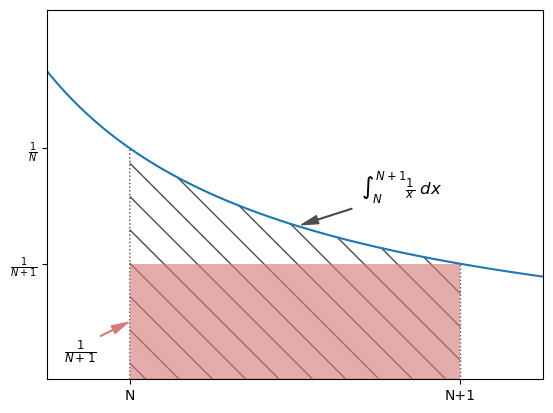
\includegraphics[scale=0.6]{rendered/euler_constant_decreasing.png}
\captionof{figure}{Area of $S_{n_1}$ and $S_{n_2}$ from $N$ to $N+1$}
\label{fig:e-const-dec}
\end{center}

Then, it is necessary to show that $S_N$ is bounded below. Under previous assertions, it is possible not only to show that it is bounded below, but also that it is contained within 0 and 1, so that $0 \leq S_N \leq 1$. \\ 
Showing that $S_N \leq 1$ is easy as it has just been proven that $S_N$ is a decreasing function. From this fact, 
\begin{align*}
    S_N &\leq S_1 \\[3 mm]
    &= \sum_{k=1}^{1} \frac{1}{k} - \int_{1}^{1}\frac{1}{x} \,dx \\[3 mm]
    &= \frac{1}{1} - 0 \\[3 mm]
    S_N &\leq 1 \\
\end{align*}
As seen in Figure \ref{fig:e-const}, showing how $S_N$ is bounded below by 0, or that $0 \leq S_N$, can also be proven geometrically as the sum of the areas of the Riemann rectangles representing $S_{n_1}$ is larger than the integral of the decreasing function $S_{n_2}$, here in red, for some interval, $1$ to $n$.
\begin{center}
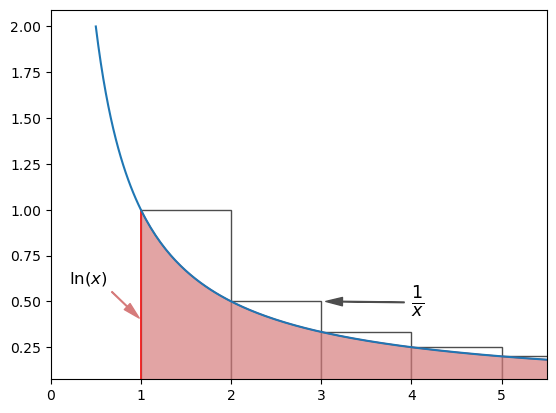
\includegraphics[scale=0.6]{rendered/euler_constant.png}
\captionof{figure}{Areas of Riemann rectangles for $S_{n_1}$ and integral of $S_{n_2}$ for some interval}
\label{fig:e-const}
\end{center}
Therefore, since the difference limiting difference between the harmonic series, $S_{n_1}$, and the natural logarithmic function,  $S_{n_2}$, is decreasing and is bounded below, it is possible to assume that it converges to a number, and this number is the the Euler-Mascheroni constant, $\gamma$.

Then, using this definition, it is possible to solve the integral of the expected value of the standard Gumbel distribution.

\begin{align*}
E(X) &= \int_{0}^{\infty} e^{-x} \ln{x} \, dx \\[3mm]
     &= \lim_{n\to \infty} \int_{0}^{n} e^{-x} \ln{x} \, dx 
\end{align*}

Using Euler's limit formula,
\begin{align*}
e^{-x}&= \lim_{n\to \infty} \left(1 - \frac{x}{n}\right)^{n} \\
      &= \lim_{n\to \infty} \int_{0}^{n} \left(1 - \frac{x}{n}\right)^{n} \ln{x} \, dx 
      & \boxed{\begin{aligned}t &= 1 - \frac{x}{n}\\
             x &= n (1-t) \\
             dx &= -n \, dt \end{aligned}} \\
      &= \lim_{n\to \infty} -n \int_{1}^{0} t^{n} \ln \left(n(1-t)\right)\, dt \\[3mm]
      &= \lim_{n\to \infty} n \int_{0}^{1} t^{n} \ln \left(n(1-t)\right)\, dt \\[3mm]
      &= \lim_{n\to \infty} n \left[ \ln{n} \int_{0}^{1} t^n \, dt + \int_{0}^{1} t^n \ln (1-t) \, dt\right] \\[3mm]
      &= \lim_{n\to \infty} n \left[ \frac{\ln{n}}{n+1} + \int_{0}^{1} t^n \ln (1-t) \, dt\right] 
      & \boxed{\begin{aligned}u &= \ln (1-t) &
             dv &= t^n \, dt \\
             du &= \frac{-1}{1-t} \, dt &
             v &= \frac{t^{n+1}}{n+1} \end{aligned}} \\[3 mm]
      &= \lim_{n\to \infty} n \left[ \frac{\ln{n}}{n+1} +  TO DO \right] 
\end{align*}


\section{Moment Generating Function}

TODO: Introduction to the moment generating function, and ...
\begin{align*}
    X & \sim \mathcal{G}\text{umbel}(0,1), \quad f(x) = e^{-(x + e^{-x})} \quad \text{ for } x \in \R \\[6mm]
    M(t) &= \E(e^{tX}) \\
         &= \lim_{(s, t)\to (-\infty, \infty)} \int_{s}^{t} e^{tx}f(x) \, dx \\
         &= \lim_{(s, t)\to (-\infty, \infty)} \int_{s}^{t} e^{tx}e^{-x - e^{-x}} \, dx \\
         &= \lim_{(s, t)\to (-\infty, \infty)} \int_{s}^{t} e^{tx - x - e^{-x}} \, dx \\
         &= \lim_{(s, t)\to (-\infty, \infty)} \int_{s}^{t} e^{-x(1-t)}e^{-e^{-x}} \, dx \\
         &= \lim_{(s, t)\to (-\infty, \infty)} \int_{s}^{t} \left(e^{-x}\right)^{-t}e^{-e^{-x}}e^{-x} \, dx
             & \boxed{\begin{aligned}u &= e^{-x} \\
             du &= -e^{-x} \, dx \end{aligned}} \\
        &= \lim_{q\to\infty} -\int_{q}^{0} u^{-t}e^{-u} \, du \\
        &= \lim_{q\to\infty}\int_{0}^{q} u^{1-t-1}e^{-u} \, du \\
        &= \Gamma(1-t) \quad \text{ for } t < 1
\end{align*}
Using the moment generating function of the standard Gumbel distribution found above, the expected value is given by
\begin{align*}
M(t)&=\Gamma(1-t) \\[3mm]
M'(t)&=-\Gamma'(1-t) \\[3mm]
M'(0)&=-\Gamma'(1) \\
    &=-(-\gamma) \\
    &= \gamma \\
    &= E(X) \\
\end{align*}
Similarly, the variance is given by
\begin{align*}
M''(t)&=-\Gamma''(1-t)(-1) \\[3mm]
M''(0)&=\Gamma''(1) \\
    &=\frac{\pi^2}{6}+\gamma^2 \\
    &= E(X^2) \\[3mm]
    \text{Var}(X)&= E(X^2)-E(X)^2 \\
    &=\frac{\pi^2}{6}+\gamma^2-(\gamma)^2 \\
    &=\frac{\pi^2}{6} \\
\end{align*}

\section{Properties}

The mode of a probability distribution is the most common value in the distribution. To determine its value, one must determine the maximum of the density function $f(x)$. To do so, it is necessary to find the point $x$ where the derivative of $f(x)$ is zero.
\begin{align*}
\frac{d}{dz}[f(x)] &= \frac{d}{dz} \left[ \frac{1}{\beta}e^{-ze^{-z}} \right] \\[3mm]
&= \frac{1}{\beta}e^{-ze^{-z}} \frac{d}{dz} \left[ -z-e^{-z} \right] \\[3mm]
&= \frac{1}{\beta}e^{-ze^{-z}} \left( -1+e^{-z} \right) =0 \\[3mm]
\end{align*}

As the exponential function is never equal to 0, $(e^{-z}-1)$ must be equal to 0.
\begin{align*}
   e^{-z}-1&=0 \\
   e^{-z}&=1 \\
   z&=0 \\
   \frac{x-\mu}{\beta}&=0 \\
   x&=\mu \\
\end{align*}

When $ X \sim \mathcal{G}\text{umbel}(\mu,\beta) $ the mode of the distribution is $\mu$.

The median of a probability distribution is the value in the middle of the density function $f(x)$. The median is located at the point $x$ where the distribution function $F(x)$ is equal to one-half. The median of the Gumbel distribution is given by

\begin{align*}
\int_{-\infty}^{x}f(u)\,du&=F(x) \\
&=\exp\left( -e^{-(x-\mu)/\beta} \right) \\
&= \frac{1}{2} \\
\ln{\left(\frac{1}{2}\right)}&=\ln{\left(\exp\left( -e^{-(x-\mu)/\beta} \right)\right)} \\[3mm]
-\ln{2}&=-e^{-(x-\mu)/\beta} \\[3mm]
\ln(\ln{2})&=\ln{\left(e^{-(x-\mu)/\beta}\right)} \\[3mm]
\ln(\ln{2})&=-\frac{x-\mu}{\beta} \\[2mm]
x&=\mu-\beta\ln{(\ln2)} \\
\end{align*}

The quantile function of a probability distribution gives the point $Q(p)$ whose probability is less than or equal to a given probability $p$. The quantile function $Q(p)$ is found by computing the inverse of the probability distribution $F(x)$. The quantile function of the Gumbel distribution is given by

\begin{align*}
F(x)=y&=\exp\left( -e^{-(x-\mu)/\beta} \right) \\
\ln{y}&=\ln{\left(\exp\left( -e^{-(x-\mu)/\beta} \right)\right)} \\[3mm]
\ln{y}&=-e^{-(x-\mu)/\beta} \\[3mm]
\ln(-\ln{y})&=\ln{\left(e^{-(x-\mu)/\beta}\right)} \\[3mm]
\ln(-\ln{y})&=-\frac{x-\mu}{\beta} \\[2mm]
x&=\mu-\beta\ln{(-\ln{y})} \\[2mm]
Q(p)&=\mu-\beta\ln{(-\ln{p})} \\
\end{align*}

The first quartile of a probability distribution is the point where the value of the distribution function is 0.25 $(p=0.25)$. The first quartile of the Gumbel distribution is given by

\begin{align*}
Q(p)&=\mu-\beta\ln{(-\ln{p})} \\
Q(0.25)&=\mu-\beta\ln{(-\ln{0.25})} \\
&=\mu-\beta\ln{(\ln{4})} \\
\end{align*}

The second quartile is the same of the median of the probability distribution.

Lastly, the third quartile of the Gumbel distribution is given by

\begin{align*}
Q(0.75)&=\mu-\beta\ln{(-\ln{0.75})} \\
&=\mu-\beta\ln{\left(\ln{\frac{4}{3}}\right)} \\
\end{align*}


\section{Applications}

Blah Blah Blah ...

\section{Logistic Distribution}

The logistic distribution gets its name from its cumulative distribution function (CDF), the logistic function.
The logistic function was discovered by Pierre François Verhulst, who used it as a model for population growth.

Verhulst derived the logistic function from the following differential equation:
\[
   \frac{dN}{dt} = rN\left(1-\frac{N}{K}\right)
\]

In this equation, $N$ is a function with respect to time, which counts the number of individuals in a population at time $t$.
The constant $r$ is known as the \textit{growth rate}, and the constant $K$ is the maximal size of the population.

Informally, the left side of the equation, $\frac{dN}{dt} = rN$, represents an exponential equation which models how
a higher number of individuals in a population leads to more offsprings. By adding the term $\left(1 - \frac{N}{K}\right)$, the
exponential growth is bounded upwards by the maximal number of individuals in the population $K$. As $N$ approaches $K$,
the above term decreases towards $0$, which  attenuates the growth. Generally, This term models the limited amount of resources
available in an environment. Solving this differential equation gives rise to the general form of the logistic function.

The standard logistic curve (Equation \ref{log:1}) is defined by the above differential equation with $r = 1$ and $K = 1$.
\begin{equation} \label{log:1}
    \frac{dN}{dt} = N(1-N)
\end{equation}
In this context, the function $N$ bounded in the range $(0, 1)$, and it
represents the proportion of the population regarding its maximal size.

The full derivation of the standard logistic function follows,
\begin{align*}
    \frac{dN}{dt} & = N(1-N) \\
    1 & = \frac{dN}{dt} \cdot \frac{1}{N(1-N)} & \frac{A}{N} + \frac{B}{1-N} & = \frac{1}{N(1-N)} \\
     & & A(1-N) + BN &= 1 \\
    & = \frac{dN}{dt} \left( \frac{1}{N} + \frac{1}{1-N} \right) & A = 1,& \quad B = 1 \\[3 mm]
    & = \frac{dN}{dt} \frac{1}{N} + \frac{dN}{dt} \frac{1}{1-N} \\[3 mm]
    \int \, dt & = \int \frac{1}{N} \frac{dN}{dt} \, dt + \int \frac{1}{1-N} \frac{dN}{dt}  \, dt \\
    t + C & = \int \frac{1}{N} \, dN + \int \frac{1}{1-N} \, dN \\[3 mm]
    & = \ln|N| - \ln|1-N| \\
    & = \ln\left|\frac{N}{1-N}\right| \\
    \frac{N}{1-N} & = e^{t + C} \\[2 mm]
    \frac{1-N}{N} & = e^{-(t + C)} \\
    \frac{1}{N} - 1 & = e^{-(t + C)} \\
    \frac{1}{N} & = 1 + e^{-(t + C)} \\
    N & = \frac{1}{1 + e^{-(t + C)}} \\
\end{align*}
Traditionally, the initial population, $N(0)$, is set to $1/2$.
\begin{align*}
    N(0) & = \frac{1}{1 + e^{-(0 + C)}} \\
    \frac{1}{2} & = \frac{1}{1 + e^{C}} \\
    1 + e^{C} & = 2 \\
    e^{C} & = 1 \\
    C & = 0
\end{align*}

Thus, the standard logistic function is given by
\begin{equation} \label{log:2}
    f(x) = \frac{1}{1 + e^{-x}}
\end{equation}

\subsection{Specification}

Throughout this section, it is assumed that $X$ follows a logistic distribution with parameters $\mu$ and $s$,
unless specified otherwise.
\[
    X \sim \mathcal{L}\text{ogistic}(\mu, s)
\]

This section is dedicated to applying some of the common properties of probability distributions to the logistic distribution.

\subsubsection{Cumulative Distribution Function}
As stated previously, the CDF of the logistic distribution is the logistic function (Equation \ref{log:2}).
In its general form, the CDF is given by
\[
   F(x) = \frac{1}{1 + e^{-\frac{x-\mu}{s}}}
\]

where $\mu$ is the location parameter and $s$ is the scale parameter.
TODO: Graph of the CDF

\subsubsection{Probability Density Function}

The PDF of the logistic distribution is trivially derived from the CDF.
\begin{align*}
    \frac{d}{dx} [F(x)] & = \frac{d}{dx} \left[\frac{1}{1 + e^{-\frac{x-\mu}{s}}}\right] \\
                      & = \frac{e^{-\frac{x-\mu}{s}}}{s(1 + e^{-\frac{x-\mu}{s}})^2} \\
\end{align*}

\begin{center}
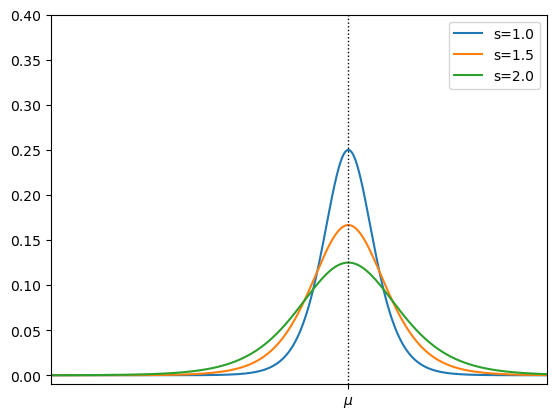
\includegraphics[scale=0.6]{rendered/logistic_density.png}
\captionof{figure}{Logistic Distribution Probability Density Function}
\label{fig:logistic-density}
\end{center}

\subsubsection{Symmetry}

The probability density function of the logistic distribution is symmetric about the location parameter $\mu$.
This property can easily be seen by observing the graph of the PDF (Figure \ref{fig:logistic-density}),
and it is trivially proven, which will be useful in subsequent derivations.

Formally, symmetry around $\mu$ denotes that $f(\mu + x) = f(\mu - x)$.
\begin{align*}
    f(\mu + x) & = \frac{e^{-\frac{\mu + x-\mu}{s}}}{s\left(1 + e^{-\frac{\mu + x-\mu}{s}}\right)^2} \\
               & = \frac{e^{-\frac{x}{s}}}{s\left(1 + e^{-\frac{x}{s}}\right)^2} \\
               & = \frac{e^{-\frac{x}{s}}}{s\left(1 + e^{-\frac{x}{s}}\right)^2} \cdot \frac{e^{\frac{2x}{s}}}{e^{\frac{2x}{s}}} \\
               & = \frac{e^{\frac{x}{s}}}{s\left(1 + e^{\frac{x}{s}}\right)^2} \\
               & = \frac{e^{-\frac{\mu - x - \mu}{s}}}{s\left(1 + e^{-\frac{\mu - x - \mu}{s}}\right)^2} \\
               & = f(\mu - x)
\end{align*}

\subsubsection{Expected Value}

One should anticipate that the expected value of the logistic distribution is $\mu$, much like how the
expected value of the normal distribution is its parameter $\mu$.

To prove this, it suffices to use the fact that the PDF of the distribution is symmetric about $\mu$.
\begin{align*}
    \E(X) & = \int_{-\infty}^{\infty} xf(x) \, dx \\
          & = -\int_{\infty}^{-\infty} (2\mu - v)f(2\mu - v) \, dv & \boxed{
              \begin{aligned}
                  v & = 2\mu - x \; \\
                  x & = 2\mu - v \\
                  \; dv & = -dx
              \end{aligned}
          } \\
          & = 2\mu \int_{-\infty}^{\infty} f(2\mu - v) \, dv - \int_{-\infty}^{\infty} vf(2\mu - v) \, dv \\
          & = 2\mu \int_{-\infty}^{\infty} f\left(\mu + (\mu - v)\right) \, dv
          - \int_{-\infty}^{\infty} vf\left(\mu + (\mu - v)\right) \, dv \\
          & = 2\mu \int_{-\infty}^{\infty} f\left(\mu - (\mu - v)\right) \, dv
          - \int_{-\infty}^{\infty} vf\left(\mu - (\mu - v)\right) \, dv & \text{(by symmetry)} \\
          & = 2\mu \cancelto{1}{\int_{-\infty}^{\infty} f(v)} - \int_{-\infty}^{\infty} vf(v) \, dv \\
          & = 2\mu - \E(X) \\
    2\E(X) & = 2\mu \\
    \E(X) & = \mu
\end{align*}

\subsubsection{Mode}

As stated previously, the mode of a probability distribution is found by maximizing the probability density function.
\[
    \mode(X) = \argmax_{x} f(x)
\]
To proceed, we first find the derivative of the PDF and equate it to zero to find critical points. It is worth noting that
the scale parameter $s$ is ignored in this derivation, as it does not affect the location of the mode,
making the derivation simpler.
\begin{align*}
    \frac{d}{dx} [f(x)] & = \frac{d}{dx} \left[ \frac{e^{-(x-\mu)}}{\left(1 + e^{-(x-\mu)}\right)^2} \right] \\
                        & = \frac{-e^{-(x-\mu)} \left(1 + e^{-(x-\mu)}\right)^{2}
                        + 2e^{-2(x-\mu)}\left(1 + e^{-(x-\mu)}\right)}{\left(1 + e^{-(x-\mu)}\right)^4} \\
                        &  = \frac{e^{-(x-\mu)}\left(- 1 - e^{-(x-\mu)} + 2e^{-(x-\mu)} \right)}{\left(1 + e^{-(x-\mu)}\right)^3} \\
                        & = \frac{e^{-(x-\mu)}\left(e^{-(x-\mu)} - 1\right)}{\left(1 + e^{-(x-\mu)}\right)^3} \\
    0 & = \frac{e^{-(x-\mu)}\left(e^{-(x-\mu)} - 1\right)}{\left(1 + e^{-(x-\mu)}\right)^3} \\
    0 & = e^{-(x-\mu)}\left(e^{-(x-\mu)} - 1\right) \\
\end{align*}
Here, $e^{-(x-\mu)}$ never equals zero, unless $x \to \infty$. Thus, the only real solution to the above equation is
\begin{align*}
    0 & = e^{-(x-\mu)} - 1 \\
    1 & = e^{-(x-\mu)} \\
    x - \mu & = 0 \\
    x & = \mu
\end{align*}
One also needs to analyze the extrema of the function to find the absolute maximum.
\begin{align*}
    \lim_{x\to\infty} f(x) & = \lim_{x\to\infty} \frac{e^{-(x-\mu)}}{\left(1 + e^{-(x-\mu)}\right)^2} \\
                           & = \lim_{x\to\infty} \frac{\cancelto{0}{e^{-x}}}{\left(1 + \cancelto{0}{e^{-x}}\right)^{\; 2}} \\
                           & = \lim_{x\to\infty} \frac{0}{1} \\
                           & = 0 \\
\end{align*}

By symmetry, the function also approaches zero as $x \to -\infty$. Morally, the maximum of the PDF cannot be zero,
since the PDF must have an area under its curve of $1$. Thus, the mode of the logistic distribution must be $\mu$,
which is visually confirmed by the graph of the PDF (Figure \ref{fig:logistic-density}).

\subsubsection{Quantile Function}

The quantile function, $Q(p)$, of a probability distribution which has a strictly monotonic CDF
can be found by inverting the CDF. The logistic distribution meets the former condition, thus its quantile function
can be derived in the following manner:
\begin{align*}
    F(x) & = \frac{1}{1 + e^{-\frac{x-\mu}{s}}} \\
    p & = \frac{1}{1 + e^{-\frac{Q(p)-\mu}{s}}} \\
    e^{-\frac{Q(p)-\mu}{s}} & = \frac{1}{p} - 1 \\
    -\frac{Q(p)-\mu}{s} & = \ln(1 - p) - \ln(p) \\
    Q(p) & = \mu - s\ln\left(\frac{p}{1-p}\right)
\end{align*}

\subsubsection{Median}

In discrete probability theory, the median refers to the "middle value," which divides the probability distribution
into two halves where any sample has an equal probability of being less than or greater than the median. In the case
of a continuous random variable, the median is the value of $x$ where $F(x) = 1/2$, or equivalently, $Q(1/2)$.
\begin{align*}
    Q(1/2) & = \mu - s\ln\left(\frac{1/2}{1-1/2}\right) \\
           & = \mu
\end{align*}

\section{Appendix}

Proof that $(1+t/n)^n=e^t$ as $n\to\infty$
\begin{align*}
y&=\left( 1+\frac{t}{n} \right)^n \\[2mm]
\ln{y}&=n\ln{\left( 1+\frac{t}{n} \right)} \\[2mm]
&=\frac{\ln{\left( 1+\frac{t}{n} \right)}}{\frac{1}{n}} \\[2mm]
\lim_{n\to\infty} \ln{y} &= \lim_{n\to\infty} \frac{\ln{\left( 1+\frac{t}{n} \right)}}{\frac{1}{n}} \quad \left[ \frac{0}{0} \right ] \text{case} \\[2mm]
&= \lim_{n\to\infty} \frac{\frac{1}{1+\frac{t}{n}}\frac{-t}{n^2}}{\frac{-1}{n^2}} \\[2mm]
&= \lim_{n\to\infty} \frac{t}{1+\cancelto{0}{\frac{t}{n}}} \\[2mm]
&=t \\[5mm]
\lim_{n\to\infty} \left( 1+\frac{t}{n} \right)^n&= \lim_{n\to\infty} y \\[2mm]
&=\lim_{n\to\infty} e^{\ln{y}} \\[2mm]
&=e^{\lim_{n\to\infty} \ln{y}} \quad (\text{as $e^{lny}$ is continuous on $\R$})\\[2mm]
&=e^t
\end{align*}

\section{Bibliography}

Blah Blah Blah ...

\end{document}
